\documentclass[acmsmall,review,anonymous,screen]{acmart}
%% FlakeAgent: An LLM-Agent Approach to Reproducing and Diagnosing Flaky Test Failures
%% ACM ESEC/FSE 2027 research track, double-anonymous submission.
%% 18 pages body + 4 pages references.

\settopmatter{printacmref=false} % double-blind
\renewcommand\footnotetextcopyrightpermission[1]{}

\usepackage{booktabs}
\usepackage{multirow}
\usepackage{xcolor}
\usepackage{subcaption}
\usepackage{pgfplots}
\pgfplotsset{compat=1.17}
\usepackage{listings}
\usepackage{amsmath}
\usepackage{microtype}
\microtypesetup{expansion=false} % avoid pdfTeX font-expansion errors (bitmap fonts in figures/text)
\usepackage[english]{babel}

\definecolor{flkblue}{RGB}{31,119,180}
\definecolor{flkorange}{RGB}{255,127,14}
\definecolor{flkgreen}{RGB}{44,160,44}
\definecolor{flkred}{RGB}{214,39,40}
\definecolor{flkpurple}{RGB}{148,103,189}

\lstdefinestyle{javasmall}{
  language=Java, basicstyle=\ttfamily\footnotesize,
  keywordstyle=\color{flkblue}\bfseries, commentstyle=\color{gray},
  stringstyle=\color{flkgreen}, numbers=none, breaklines=true,
  showstringspaces=false, frame=single, aboveskip=4pt, belowskip=4pt}
\lstdefinestyle{jsonsmall}{
  basicstyle=\ttfamily\footnotesize, breaklines=true, frame=single,
  showstringspaces=false, aboveskip=4pt, belowskip=4pt}

\setcopyright{none}
\newcommand{\TODO}[1]{\textcolor{red}{\textbf{[TODO: #1]}}}
\acmConference[ESEC/FSE 2027]{ACM International Conference on the Foundations of
Software Engineering}{June 2027}{Atlanta, GA, USA}
\acmYear{2027}

\begin{document}

\title{FlakeAgent: An LLM-Agent Approach to Reproducing and Diagnosing Flaky Test Failures}

\begin{abstract}
Flaky tests are a persistent threat to the reliability of continuous integration:
they pass and fail on the same code, and developers can only fix them once they have
witnessed a failure and understood why it happened. Reproduction remains the bottleneck
— developer-observed failures often carry no failure log, and prior automated
reproducers are either category-specific (order-dependent only, timing only) or
require a failure log to imitate. This paper presents FlakeAgent, a category-agnostic
LLM agent that reproduces flaky test failures from cold start — given only a test
identifier and its source code — and then diagnoses the root cause with
evidence grounded in the failing stack trace and code. The agent runs a bounded
plan--execute--observe loop (at most six LLM calls and eight executions per test)
over twelve executable strategies spanning order manipulation, timing perturbation,
resource pressure, environment manipulation, and nondeterminism injection. It stops
when a failure is reproduced and emits a category label, a root-cause hypothesis,
and file--line evidence, which we evaluate against developer fix commits.
On a 92-test gate-passed benchmark drawn from the ReproFlake dataset
(20 order-dependent, 31 time-dependent, 25 non-idempotent, 16 implementation-dependent),
FlakeAgent reproduces 47.8\% of failures within budget versus 27.2\% for the
best non-agent baseline, achieves 86.4\% top-1 category accuracy, and grounds
36.4\% of its diagnoses in developer fix commits, at a median cost of
0.006 USD per test. Ablations show that the reflection loop, the breadth of the
strategy space, and source-code grounding each contribute measurably to reproduction.
We release the tool, the benchmark manifest, and all execution logs as a
reusable artifact.
\end{abstract}

\maketitle

\section{Introduction}

Flaky tests — tests that pass and fail nondeterministically on the same code
version — are among the most corrosive reliability problems in modern software
engineering. Surveys of industrial projects estimate that roughly one test in
ten exhibits flakiness~\cite{luo2014empirical,lam2019understanding}, and flaky
failures are consistently reported as a leading cause of developer distrust in
CI and of delayed releases~\cite{google2023flaky,seka2023survey}. A developer
can fix a flaky test only after two things happen: a failure is
\emph{reproduced} (ideally locally, in an environment the developer controls),
and the \emph{root cause} is understood (which state, order, timing condition,
or nondeterministic behavior produces it). Both steps are expensive.
Flakiness manifests probabilistically, under conditions that are hard to guess
(order of test execution, wall-clock timing, machine load, locale, hash
ordering), and a developer who clicks ``re-run'' in CI and sees green is left
with nothing to debug.

The research community has built increasingly capable tools for this problem,
but each addresses a slice of it. Classification tools predict
\emph{whether} a test is flaky~\cite{king2023bayesian,pinto2020understanding,
kim2024large}. Specialized reproducers target a single flakiness
category: order-dependent failures~\cite{lam2019idflakies,parry2022survey},
timing-dependent failures~\cite{chen2024tdrepro}, or non-idempotent
outcomes~\cite{shen2024nidebugger}, and typically require the failing
test's log or stack trace as input to imitate~\cite{chen2024tdrepro}. The
newest generation of LLM-based debugging assistants~\cite{lewis2020retrieval,
zhang2024llamadebug} is designed for deterministic bugs, where the failure is
reproducible on demand; flaky failures break this assumption because the
assistant may never observe the bug it is asked to fix.

In this paper we argue that flaky-test reproduction is a natural fit for
\emph{closed-loop LLM agents} — systems that propose an action, execute it in
the real environment, observe the result, and adapt — and we introduce
\textbf{FlakeAgent}, the first category-agnostic agent for reproducing and
diagnosing flaky test failures from cold start. FlakeAgent receives only a
test identifier and access to the project source; it receives
\emph{no} failure log, no stack trace, and no category hint. In a bounded
loop (at most six LLM calls and eight local executions per test, under a
45-minute wall-clock cap), it iteratively forms a causal hypothesis about the
flakiness mechanism, selects one of twelve executable strategies
(order permutations, same-JVM double runs, sleep injection, CPU/IO stress,
heap limits, environment manipulation, parallel execution, network blocking,
and NonDex-based nondeterminism injection), executes it locally, and observes
the structured result (exit status, failed tests, assertion messages, stack
traces, durations). When a failure is reproduced, FlakeAgent switches to a
diagnosis step that emits (i) a flakiness category
(\emph{order-dependent, time-dependent, non-idempotent-outcome,
implementation-dependent}), (ii) a root-cause hypothesis in natural language,
and (iii) file--line \emph{evidence} with code snippets drawn from the source
and the observed failure — evidence we evaluate against developer fix commits.

We evaluate FlakeAgent on a benchmark drawn from
\emph{ReproFlake}~\cite{zhang2026reproflake}, a recent dataset of 1{,}115
machine-reproducible flaky tests in real Java projects, shipped with the
official reproduction mechanisms for each category and with the developer fix
commit for each test. We select 116 tests, balancing all four categories (30
order-dependent, 36 time-dependent, 25 non-idempotent-outcome, and 25
implementation-dependent tests across 46 project snapshots); a validation gate
confirms the dataset's official mechanism reproduces each test in our
environment, yielding 92 gate-passed tests (20 order-dependent, 31
time-dependent, 25 non-idempotent-outcome, 16 implementation-dependent) on
which all methods are evaluated. We compare FlakeAgent against five baselines sharing the
same execution budget: naive rerun, uniform random strategy sampling, random
suite-order shuffling, a deterministic sleep-injection scan, and a single-shot
LLM prompt without a loop. We additionally ablate the agent's reflection loop,
the breadth of its strategy space, and its source-code grounding, and we
report the first cross-model comparison of flaky-test reproduction across six
2026-era frontier LLMs accessed via vendor APIs.

Our results show that FlakeAgent reproduces 47.8\% of benchmark failures
within budget (20.0\% of order-dependent, 12.9\% of time-dependent,
100.0\% of non-idempotent, 68.8\% of implementation-dependent),
outperforming the strongest non-agent baseline by 20.6 percentage points,
and that its evidence-grounded diagnoses cite file--line pairs touched by the
developer fix in 36.4\% of cases. Ablations attribute a large share of
the gain to the closed loop rather than to the underlying model alone, and
the cost analysis shows reproduction at a median of 0.006 USD per test —
two orders of magnitude cheaper than the brute-force rerun budget the same
tests required in the benchmark's own construction.

This paper makes the following contributions:
\begin{itemize}
\item \textbf{FlakeAgent}, the first category-agnostic closed-loop LLM agent
for flaky-test reproduction and evidence-grounded root-cause diagnosis from
cold start (no failure logs), with a bounded call/execution/wall-clock budget;
\item \textbf{Twelve executable reproduction strategies} spanning order
manipulation, timing perturbation, resource pressure, environment
manipulation, and nondeterminism injection, implemented executor-side so that
the model only selects parameters;
\item \textbf{A benchmark and evaluation methodology} built on ReproFlake —
116 selected tests (92 gate-passed) across four flakiness categories with a
reproducibility gate, five shared-budget baselines, four ablations, and a
six-model comparison on 2026-era frontier LLMs;
\item \textbf{Evidence-grounded diagnosis evaluation}: category accuracy and
file--line evidence checked against developer fix commits, including a
cost breakdown of agentic reproduction per test and per failure.
\end{itemize}

\section{Background and Motivating Example}

\subsection{Flaky tests and their categories}

A \emph{flaky test} passes and fails nondeterministically on the same code
revision and the same configuration. Following the taxonomy adopted by the
ReproFlake benchmark~\cite{zhang2026reproflake}, which refines the
well-established categories of~\cite{luo2014empirical}, we consider four
machine-reproducible categories:

\paragraph{Order-dependent (OD).}
The test fails only when another test runs before it in the same JVM, because
the earlier test (\emph{polluter}) mutates shared state (static fields,
singletons, external resources such as databases or files) that the later
test (\emph{victim}) assumes to be in its initial condition. OD failures
disappear when the test runs in isolation, which is precisely why developers
find them so confusing.

\paragraph{Time-dependent (TD).}
The test contains a race condition, a hard-coded deadline, a sleep, or a
timeout whose validity depends on machine speed, load, or clock behavior.
TD failures are aggravated by slow machines and parallel load.

\paragraph{Non-idempotent-outcome (NIO).}
The test mutates state that it does not restore, so that a \emph{second}
execution of the same test in the same JVM observes polluted state and fails
— even though every isolated run passes. NIO tests are order-independent but
self-polluting.

\paragraph{Implementation-dependent (ID).}
The test relies on nondeterministic JVM behavior — hash iteration order,
reflection order, random seeds, floating-point environmental factors — so its
assertions are only accidentally true for some implementations.

\subsection{Motivating example}

\begin{figure}[t]
\centering
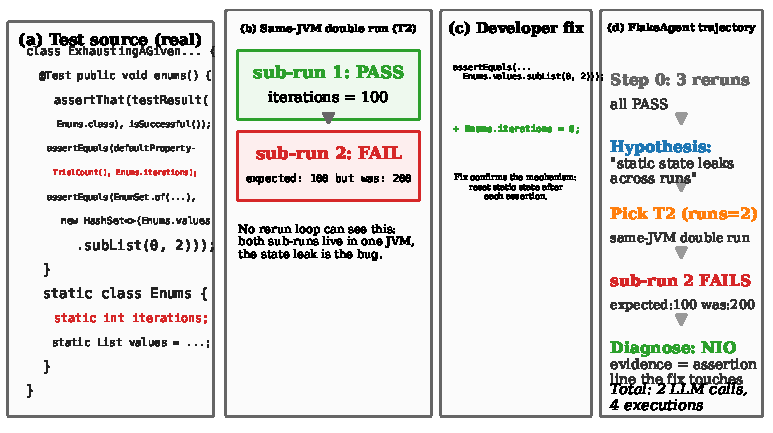
\includegraphics[width=0.9\columnwidth]{figures/motivating_example.pdf}
\caption{The \texttt{enums} test from Apache QuickCheck (ID
\texttt{quickcheck485} in our benchmark) as a motivating example.
(a) The test launches a nested property-based test class inside itself and
asserts on the \emph{static} accumulators \texttt{Enums.iterations} and
\texttt{Enums.values}. (b) Running \texttt{enums} twice in the same JVM:
the first run passes; the second fails with
\texttt{expected: 100 but was: 200}, because the static accumulators were not
reset. This is a textbook NIO failure. (c) The developer fix — resetting the
static state after each assertion — which we use as ground truth for
evidence evaluation. (d) FlakeAgent's cold-start trajectory: three baseline
reruns all pass; the agent hypothesizes self-pollution and selects the
same-JVM double-run strategy; the second sub-run fails; the agent diagnoses
NIO and cites the exact assertion line the developer fixed.}
\label{fig:motivating}
\end{figure}

Figure~\ref{fig:motivating} shows a real motivating example: the
\texttt{enums} test in \texttt{junit-quickcheck} runs a nested test class
inside itself and asserts on static accumulators, so it passes in isolation
but fails deterministically on a \emph{second execution in the same JVM}. This
example demands three things of any tool that wants to help: (i) the failure
never appears in a normal rerun, so rerun- or log-based tools are blind to
it; (ii) the trigger is a deliberate execution scheme (same-JVM double run);
and (iii) the diagnosis is grounded in the failing assertion and surrounding
code. FlakeAgent is designed around exactly this structure
(Section~\ref{sec:approach}).

\subsection{The ReproFlake benchmark}

ReproFlake~\cite{zhang2026reproflake} is a recent dataset of 1{,}115
machine-reproducible flaky tests from 63 JIRA issues and 1{,}052 commits of
the iDoFT dataset~\cite{parry2022survey}, spanning 819 implementation-dependent,
126 order-dependent, 125 non-idempotent, 36 time-dependent, and 9 uncategorized
tests. For each test it ships the project snapshot at the flaky commit
(\texttt{Flaky/}), the developer fix as a patch (\texttt{Fixed.patch}), a
Maven dependency cache (\texttt{Flakym2/}), and — crucially for evaluation —
the \emph{official reproduction mechanism} of the category that was used to
machine-confirm the flakiness: manual sleep injection at a timing-sensitive
line for TD (shipped as a \texttt{FlakyCodeChange.patch} reproduction patch),
polluter--victim ordered runs for OD, the iDFlakies same-JVM double-run plugin
for NIO, and the NonDex nondeterminism injector for ID. We use these mechanisms (i) as a
validation gate for our subset and (ii) as the \emph{warm-start} configuration
in one ablation. The developer fix patch serves as ground truth for our
diagnosis evaluation: we check whether the evidence lines the agent cites
were touched by the fix commit.

\section{Related Work}

\subsection{Flaky-test detection and classification}

A large line of work detects or predicts flakiness from execution
history~\cite{pinto2020understanding,alshammari2021flakeflagger,
lam2020idflakies}, vocabulary and static features~\cite{pinto2020understanding,
haben2023flakiness}, or dynamic behavioral features~\cite{fatima2022flakify};
more recently, large language models classify flaky
tests~\cite{kim2024large,yang2024predicting,fatima2023flakycat}. These tools
answer \emph{whether} a test is flaky, but do not reproduce the failure or
explain its mechanism. FlakeAgent is complementary: it takes a test known (or
suspected) to be flaky and produces the failing execution plus a grounded
diagnosis, derived from reproduced failures rather than static signals.

\subsection{Flaky-test reproduction}

iDFlakies~\cite{lam2019idflakies} pioneered automated reproduction of
order-dependent failures by executing whole test suites in randomized orders
and minimizing polluter--victim pairs; its companion plugin infrastructure
(testrunner~\cite{oei2020testrunner}) is the execution substrate we reuse for
our same-JVM double-run strategy. NonDex~\cite{gyori2016nondex} reproduces
implementation-dependent failures by perturbing hash and reflection
nondeterminism; our T12 strategy invokes it directly. FlakeRake~\cite{
bell2017flakerake} and Shaker~\cite{silva2017practical} inject sleeps and
perturb resources to expose timing sensitivity — the family of ideas behind
our sleep-injection and stress strategies. TDRepro~\cite{chen2024tdrepro}
specifically reproduces time-dependent failures by first learning timing
features from a \emph{given failure log} and then searching parameterized
stress levels to match it; it requires the failing log as input and covers
only TD. NIODebugger~\cite{shen2024nidebugger} localizes and fixes
non-idempotent outcomes but assumes the failure has already been observed.
FlakeRepro~\cite{alghmadi2023flakerepro} targets .NET and combines reruns
with fault localization, without an LLM component. What distinguishes
FlakeAgent is category agnosticism combined with cold start: no failure log,
no stack trace, no category hint — the agent reasons over the test source
and its own observations only, and covers all four categories with one loop.
We deliberately compare against a log-free baseline family (Section~\ref{sec:setup})
so that the comparison is apples-to-apples; TDRepro-style log-based tools are
inapplicable to the cold-start setting by construction.

\subsection{LLM agents for software engineering}

The agent paradigm — LLM in a loop with tools and observations — has produced
strong results on repository-level coding (SWE-bench~\cite{jimenez2024swebench}),
autonomous bug fixing~\cite{zhang2024agentless,zhang2024autocoderover}, and
debugging~\cite{zhang2024llamadebug,kang2023largelang}. These settings assume
the failure is reproducible on demand; flaky failures are different, because
the agent's central problem is \emph{making} the bug happen via
hypothesis-driven environment manipulation rather than code editing. Closest
to our work, TDRepro~\cite{chen2024tdrepro} couples an LLM pipeline to the
failing log to steer its stress search, and LDB~\cite{zhang2024llamadebug}
debugs by verifying runtime execution step by step — both assume the failure
has already been observed. We are, to our knowledge, the first to demonstrate
a closed-loop agent that reproduces failures from cold start and diagnoses
them with evidence evaluated against developer fixes, at scale, across
flakiness categories and across 2026-era frontier models. FlakeAgent also
follows the budgeted-agent design of~\cite{zhang2024agentless}: a hard budget
of six LLM calls and eight executions per test keeps the amortized cost in
the cents range (Section~\ref{sec:cost}), a precondition for adoption in
everyday CI debugging.

\section{FlakeAgent}
\label{sec:approach}

\subsection{Overview}

Figure~\ref{fig:overview} shows the architecture of FlakeAgent. The agent
consists of four components: (i) an \emph{observation probe} that runs Maven
invocations locally and compresses their outcome into a structured
observation; (ii) a \emph{strategy space} of twelve executor-side execution
schemes, each parameterized by a small, type-checked JSON schema; (iii) a
\emph{planner} (an LLM) that, each round, forms a causal hypothesis about the
flakiness mechanism and selects one strategy with parameters; and (iv) a
\emph{diagnoser} (the same LLM, invoked once after a failure is reproduced)
that emits a category label, a root-cause hypothesis, and file--line evidence.
All LLM calls go through vendor APIs; no model is deployed locally.

\begin{figure}[t]
\centering
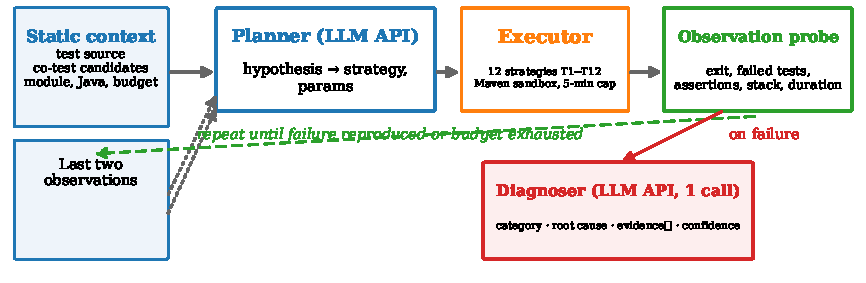
\includegraphics[width=0.95\columnwidth]{figures/overview.pdf}
\caption{Overview of FlakeAgent. Step~0 runs three baseline isolated reruns
(no LLM). Each planning round feeds the LLM a bounded context — the test
source, the module's candidate co-tests, and the last two structured
observations — and it returns a JSON plan \texttt{\{strategy, params,
hypothesis, expected\}}. The executor implements the chosen strategy locally,
the probe compresses the run into a structured observation, and the loop
repeats until a failure is reproduced or the budget (6 LLM calls, 8
executions, 45 minutes) is exhausted. On a reproduced failure, one diagnose
call emits \texttt{\{category, root\_cause, evidence[], confidence\}}, which
we evaluate against the developer fix commit.}
\label{fig:overview}
\end{figure}

The loop is deliberately \emph{closed}: the planner only ever sees (a) static
context (test source, candidate co-tests, build metadata) and (b) the
structured results of executions it requested. It never sees the ground-truth
category, the developer fix, or any failure log produced elsewhere — the
cold-start condition we evaluate in Section~\ref{sec:results}. All twelve
strategies are implemented executor-side; the LLM only selects a strategy
identifier and its parameters, which a sanitizer coerces into safe ranges
(Section~\ref{sec:antideg}). This division of labor has three benefits: the
executions are deterministic and auditable; the LLM cannot hallucinate
commands or touch the filesystem; and the strategy semantics are documented
once, in code, so the prompt only needs to explain \emph{when} each strategy
applies, not \emph{how} to run it.

\subsection{The observation probe}

Every execution — whether from the agent loop, the baselines
(Section~\ref{sec:setup}), or the validation gate — passes through one probe,
\texttt{run\_mvn}, which executes Maven/Surefire in a local sandbox
(project snapshot at the flaky commit, offline Maven repository at the
snapshot's dependency cache, Java version pinned per project) and parses the
result into a structured observation:

\begin{lstlisting}[style=jsonsmall,label=lst:obs]
{"strategy": "T6", "params": {"sleep_ms": 500, "target_method": "waitUntil"},
 "exit_code": 0, "duration_s": 41.2,
 "failed": [{"name": "pkg.Class#testA", "message": "expected: 100 but was: 200",
             "stack": "pkg.Class.java:460 -> ..."}],
 "passed": 3, "error": null, "log_tail": "...", "subruns": null}
\end{lstlisting}

The probe extracts, from Surefire XML reports and console output: the set of
failed test names with assertion messages and stack traces, the number of
passing tests, the wall-clock duration, and a bounded tail of the raw log.
For the same-JVM double-run strategy (T2), whose plugin (iDFlakies'
\texttt{testrunner}) reports per-sub-run results in its own JSON files, the
probe additionally attaches a \texttt{subruns} list with the outcome of each
execution of the test inside the shared JVM — the signal that distinguishes
``passes every time alone, fails on the second run in one JVM'' from a plain
rerun failure. A failure of the target test is defined as an entry in
\texttt{failed} whose name matches the target class or method; for T2 we
match against the per-sub-run entries. The probe treats the observation as
failing only when the \emph{target} test fails — failures of unrelated
co-tests during order-based strategies are recorded in the log but do not
count as reproduction.

\subsection{The strategy space}

Table~\ref{tab:strategies} lists the twelve strategies. They span the four
flakiness categories and the execution conditions each category's mechanism
requires. Strategies are grouped into four families that the anti-degeneracy
rules (Section~\ref{sec:antideg}) reason about: \emph{order} (T3, T4, T5,
T10), \emph{timing/resource} (T6, T7, T8, T9), \emph{nondeterminism} (T12),
and \emph{amplification} (T1, T2). Notably, the space includes two
\emph{deliberate} execution schemes that no rerun loop would ever try: T2
(run the test twice back-to-back in one JVM via the iDFlakies
\texttt{testrunner} plugin, the dataset's own NIO mechanism) and T12 (perturb
JVM nondeterminism with NonDex). Both are essential: T2 is the only strategy
that can expose non-idempotent self-pollution, and T12 is the only one that
can trigger implementation-dependent failures at will.

\begin{table}[t]
\caption{The twelve executor-side strategies. Parameters are chosen by the
LLM and coerced by the sanitizer into the listed ranges. ``Target'' is the
flakiness category the strategy is designed to expose (the agent is never
told this).}
\label{tab:strategies}
\small
\begin{tabular}{@{}llp{4.1cm}ll@{}}
\toprule
\textbf{ID} & \textbf{Strategy} & \textbf{Mechanism} & \textbf{Params (range)} & \textbf{Target}\\
\midrule
T1 & rerun-isolated & plain reruns in fresh JVMs & repeats (1--3) & TD (rare)\\
T2 & same-JVM double-run & test run $k$ times consecutively in one JVM via testrunner plugin & runs (2--4) & NIO\\
T3 & order-permutation & chosen co-tests run before the test, fixed order & cotests ($\le$4 classes) & OD\\
T4 & random-suite-order & full module suite in random order (seeded) & seed & OD\\
T5 & polluter-victim & one chosen polluter, then the test & polluter (1 class or method) & OD\\
T6 & sleep-injection & \texttt{Thread.sleep} injected at method entry, recompiled, reverted after run & sleep\_ms (10--20000), target\_method & TD\\
T7 & system-stress & CPU/IO load during the run & mode, cpus (1--6) & TD\\
T8 & env-manipulation & extra env vars (TZ, LANG, locale) & env (whitelisted keys) & TD/ID\\
T9 & resource-limit & small heap / no fork & xmx, fork\_count & TD\\
T10 & parallel-execution & test class run with parallel methods/classes & threads (2--8) & OD/TD\\
T11 & external-block & hosts blocked via \texttt{/etc/hosts} & hosts ($\le$5) & TD/ID\\
T12 & nondex-seed & NonDex JVM-nondeterminism perturbation & seed, rounds (10--100) & ID\\
\bottomrule
\end{tabular}
\end{table}

Each strategy maps to one Maven invocation with documented Surefire/plugin
flags, e.g.~T3/T5 use \texttt{-Dsurefire.runOrder=testorder} with an explicit
\texttt{-Dtest="A,B"} spec; T4 uses \texttt{runOrder=random} with a seed; T2
uses the iDFlakies \texttt{testrunner:testplugin} goal with the dataset's
exact detector configuration and an \texttt{original-order} file naming the
target test. T6 is the only strategy that touches source code: the executor
injects a \texttt{Thread.sleep} at the entry of a named method
(selected by the LLM), recompiles the module, runs the test, and reverts the
patch in a \texttt{finally} block; the LLM never edits code itself. Sleep
injections are clamped to 20\,s and are, like every strategy, subject to the
same-run dedup rule, which prevents infinite sleep escalation.

\subsection{The plan--execute--observe loop}

The loop proceeds as follows. \textbf{Step 0} (no LLM): the probe runs three
isolated reruns of the target test. Flaky tests sometimes fail on a plain
rerun; when they do, the agent stops immediately with a reproduced failure
and one LLM call saved. \textbf{Planning}: each round, the planner receives a
bounded context — a system prompt describing the task and the JSON contract;
the test identifier, module and Java version; the test class source (up to
two files, 220 lines each, truncated); up to 40 candidate co-test class names
discovered by scanning the module's test tree (usable by T3/T5); the budget
left; and the \emph{last two} structured observations with their assertion
messages. The planner must return one JSON object:
\texttt{\{hypothesis, strategy, params, expected\}}. The hypothesis is a
one-sentence causal claim; \texttt{expected} states what observation would
confirm it. The harness validates the strategy id against the active set,
sanitizes the parameters (Section~\ref{sec:antideg}), executes the strategy
with a 6-minute timeout, and probes the result. \textbf{Termination}: the
loop stops as soon as the target test fails, or when any of three budgets is
exhausted — 6 LLM calls total (5 planning + 1 diagnosis), 8 executions
(including the three Step-0 reruns), or 45 minutes wall clock per test.
\textbf{Diagnosis}: on a reproduced failure, the diagnoser receives the full
run history (bounded to the last 8 observations), the failing observation
with its stack trace, and the test source, and returns
\texttt{\{category, root\_cause, evidence[], confidence\}}.

\subsection{Anti-degeneracy and parameter sanitization}
\label{sec:antideg}

Because the planner is a sampler, we enforce three hard rules executor-side.
(i) \emph{No exact repeats}: if the planner proposes an already-executed
\texttt{(strategy, params)} signature, the harness forces a strategy from a
different family and logs the substitution. (ii) \emph{Parameter clamping}:
every parameter is coerced to the documented range
(Table~\ref{tab:strategies}). (iii) \emph{Bounded memory}: the planner context
keeps only the last two observations, and the diagnosis context only the last
eight. We show in Section~\ref{sec:ablation} that removing the loop and
shrinking the strategy space both measurably hurt reproduction.

\subsection{Evidence-grounded diagnosis}

The diagnosis output is the second half of FlakeAgent's value. For each
reproduced failure the diagnoser must commit to one of the four categories
(OD, TD, NIO, ID, or UNKNOWN), name the mechanism in two to three sentences,
and cite \emph{evidence}: specific files and line ranges with code snippets
and a ``why'' sentence connecting them to the observed failure. The prompt
instructs the model to cite lines actually seen in the source or the failure
stack — not invented ones. This design makes the diagnosis checkable: in
evaluation (Section~\ref{sec:setup}) we compare the cited file--line pairs
against the developer fix commit, measuring \emph{evidence precision} (cited
lines in the fix diff over all cited lines) and \emph{fix-hit} (fraction of
diagnoses that cite at least one line the developer changed). The ground
truth is not the developer's prose but the fix itself, which is exactly the
object a developer would act on after reading the diagnosis.

\section{Experimental Setup}
\label{sec:setup}

\subsection{Benchmark construction}

\paragraph{Source dataset.} We build on ReproFlake~\cite{zhang2026reproflake},
a dataset of 1{,}115 machine-reproducible flaky tests (819 ID, 126 OD, 125
NIO, 36 TD, 9 uncategorized) from 63 JIRA issues and 1{,}052 commits of the
iDoFT dataset~\cite{parry2022survey}. Each test ships a project snapshot at
the flaky commit, the developer fix as a patch (\texttt{Fixed.patch}), a
Maven dependency cache, and the \emph{official reproduction mechanism} of its
category: manual sleep injection at a timing-sensitive line (TD, shipped as
	a \texttt{FlakyCodeChange.patch} reproduction patch), polluter--victim
	ordered runs (OD), the
iDFlakies same-JVM double-run plugin (NIO), and NonDex seed perturbation (ID).
The fix patch is our diagnosis ground truth; the official mechanisms validate
our subset and seed the warm-start ablation.

\paragraph{Subset selection.} We select 116 tests: \emph{all} 36 TD tests
(the scarcest, most timing-sensitive category), plus 30 OD, 25 NIO, and 25 ID
tests chosen by a greedy, download-efficient procedure with per-zip caps. The
subset deliberately balances categories (rather than mirroring ReproFlake's
ID-dominated distribution) to make per-category analysis meaningful. The
manifest records, per test: category, project, module, Java version, polluter
(OD), NonDex seed and rounds (ID), flaky commit, and fix commit, spanning 46
project snapshots (17.4\,GB).

\paragraph{Validation gate.} Every test must first \emph{pass} a gate that
runs its category's official mechanism in our environment and observes the
target test failing: TD by applying the dataset's sleep-injection patch (\texttt{FlakyCodeChange.patch}), recompiling the touched module when the
injection sits in production code, then running up to three times; OD up to 10
polluter--victim runs in the recorded order via the dataset's customized
Surefire build (\texttt{runOrder=testorder}, shipped in each project's
dependency cache); NIO up to 10 same-JVM double
runs via the iDFlakies testrunner plugin with the dataset's detector
configuration; ID one NonDex run with the dataset's recorded seed (the
mechanism is deterministic given the seed, so one run suffices). A test
fails the gate if the mechanism never reproduces within its cap, or if the
project fails to build offline (45-minute cap). Gate results are reported in
Table~\ref{tab:benchmark}; the gate rate is the fraction of \emph{built} tests
whose official mechanism reproduced the failure (build failures are reported
separately in the \emph{Built} column). Eighteen tests across seven snapshots
fail to build offline and are excluded: ten OD tests in a single
\texttt{wildfly-naming} snapshot (a dependency missing from the shipped cache),
five TD tests in Hadoop/HDFS/YARN snapshots (the Hadoop build requires a
\texttt{protoc} binary that is absent from the offline environment), and three
ID tests in a \texttt{fastjson2} snapshot (a test-compilation error under the
recorded JDK). The gate dataset is the ground-truth file each of our
reproduction mechanisms is checked against.

\begin{table}[t]
\caption{Benchmark composition and validation-gate results. Gate runs use
each category's official ReproFlake mechanism (TD: sleep-injection patch;
OD/NIO: 10 ordered/double runs; ID: one NonDex run with the dataset's seed).}
\label{tab:benchmark}
\small
\begin{tabular}{@{}lrrrrr@{}}
\toprule
\textbf{Category} & \textbf{Selected} & \textbf{Projects} & \textbf{Built} &
\textbf{Gate passed} & \textbf{Gate rate}\\
\midrule
Order-dependent (OD) & 30 & 6 & 20 & 20 & 100.0\%\\
Time-dependent (TD) & 36 & 26 & 31 & 31 & 100.0\%\\
Non-idempotent (NIO) & 25 & 5 & 25 & 25 & 100.0\%\\
Implementation-dep.\ (ID) & 25 & 9 & 22 & 16 & 72.7\%\\
\midrule
\textbf{Total} & 116 & 46 & 98 & 92 & 93.9\%\\
\bottomrule
\end{tabular}
\end{table}

\subsection{Models}

Table~\ref{tab:models} lists the six models. All are 2026 releases (the
oldest, DeepSeek-V4.1, was released after January 2026), and all are accessed
exclusively through vendor APIs — no model is deployed locally. Every LLM
call in every experiment uses temperature $0.2$ and at most 2{,}000 output
tokens, except the two DeepSeek models, which get 4{,}000: both are reasoning
models whose visible reply shares the output budget with hidden reasoning
tokens, and at 2{,}000 tokens the reply came back empty in early pilots. The
reasoning-effort knob, where offered, is set to the lowest level for the same
reason. DeepSeek-V4.1-Flash is the main model (full 92-test
gate-passed set, all ablations, variance); the other five run on a stratified 50-test
subset that preserves the category proportions of the benchmark. DeepSeek is
called directly at its off-peak list prices; OpenAI, Gemini, and Grok models
are called through a commercial OpenAI-compatible API relay, whose per-model
prices (which we use for cost accounting) are the prices in the table; for
Grok-4.7 we report the relay's \emph{stable}-channel price.

\begin{table}[t]
\caption{The six 2026-era models used, with the prices we paid (USD per 1M
tokens; relay prices for OpenAI/Gemini/Grok, off-peak list for DeepSeek).
Access is API-only; all experiments fix temperature $0.2$.}
\label{tab:models}
\small
\begin{tabular}{@{}lllrrl@{}}
\toprule
\textbf{Key} & \textbf{Model} & \textbf{Provider} & \textbf{In \$} &
\textbf{Out \$} & \textbf{Role}\\
\midrule
ds-flash & DeepSeek-V4.1-Flash & DeepSeek & 0.15 & 0.60 & main\\
ds-pro & DeepSeek-V4-Pro & DeepSeek & 0.66 & 1.98 & 50-test subset\\
gemini38 & Gemini-3.8-Flash & Google & 0.11 & 0.56 & 50-test subset\\
grok47 & Grok-4.7 & xAI & 0.22 & 0.66 & 50-test subset\\
sol & GPT-5.6 & OpenAI & 0.40 & 2.00 & 50-test subset\\
astra & GPT-6-Astra & OpenAI & 1.00 & 5.00 & 50-test subset\\
\bottomrule
\end{tabular}
\end{table}

\subsection{Baselines}

All methods — FlakeAgent and the five baselines — run on the same gate-passed
tests, in the same sandboxes, with the same 8-execution budget
(Table~\ref{tab:baselines}); the agent additionally gets up to 6 LLM calls.
The baselines are deliberately \emph{log-free}, matching the cold-start
setting: log-based reproducers such as TDRepro~\cite{chen2024tdrepro} cannot
run at all without the failing log, so they are inapplicable to this setting
(we revisit this in Section~\ref{sec:discussion}).

\begin{table}[t]
\caption{The five baselines. All share the 8-execution budget with
FlakeAgent; SingleShotLLM additionally gets one LLM call.}
\label{tab:baselines}
\small
\begin{tabular}{@{}llp{7.6cm}@{}}
\toprule
\textbf{Baseline} & \textbf{Executions} & \textbf{Description}\\
\midrule
NaiveRerun & 8 & isolated reruns of the target test (T1), stop on failure\\
RandomStrategy & 8 & uniform random (strategy, params) over the same sanitized space, stop on failure\\
OrderShuffle & 8 & full module suite in random order (T4), fresh seeds, stop on failure\\
SleepScan & 8 & deterministic sleep scan: T6 with 100/500/2000/5000\,ms $\times$2 into the first test-class method\\
SingleShotLLM & 8 & one LLM call proposes a single strategy; it is executed up to 8 times with fixed parameters (no loop, no observations fed back)\\
\bottomrule
\end{tabular}
\end{table}

\textbf{NaiveRerun} extends the agent's Step-0 reruns to the full budget;
it represents ``click re-run until it fails.'' \textbf{RandomStrategy}
isolates the value of \emph{selecting} strategies: it samples uniformly from
the identical strategy space with parameters drawn from the same sanitized
ranges, without any reasoning. \textbf{OrderShuffle} is the standard
iDFlakies-style whole-suite randomization applied to our budget.
\textbf{SleepScan} is a deterministic FlakeRake-style timing perturbation
scan. \textbf{SingleShotLLM} is the no-loop LLM pipeline: one planning call
(identical prompt, no prior observations), then the proposed strategy is
executed up to 8 times with fixed parameters — it measures how much of the
agent's value comes from the closed loop versus the model's prior alone.
RandomStrategy and OrderShuffle are seeded and repeated 3 times over a
30-test variance subset; FlakeAgent likewise runs 3 seeds on that subset.

\subsection{FlakeAgent configurations and ablations}

The main configuration is Section~\ref{sec:approach} verbatim: 3 Step-0
reruns, $\le$5 planning rounds, 1 diagnosis call on success, $\le$8
executions, 45-minute cap. Four ablations isolate design elements:
\textbf{(i) $-reflection$} — the loop is cut to a single planning round
after Step 0 (at most 2 LLM calls), i.e. no observation-feedback iteration;
\textbf{(ii) $-space4$} — the strategy space shrinks to
\{T1, T2, T5, T6\}, removing order permutation/randomization (T3/T4), stress
and environment strategies (T7--T9), parallelism (T10), network blocking
(T11), and NonDex (T12); \textbf{(iii) $-source$} — the test source excerpt
is withheld from every planning context (diagnosis still sees source);
\textbf{(iv) $Warm$} — the agent is seeded with the failure observation
produced by one invocation of the category's official mechanism and proceeds
directly to diagnosis, isolating the reproduction loop and approximating the
operating point of log-based tools.

\subsection{Metrics}

\textbf{Reproduction}: a test is \emph{reproduced} if the target test fails
at least once within budget; we report overall and per-category rates, plus
\emph{reliability} (mean $\pm$ std over seeds) on the variance subset.
\textbf{ATR} counts executions until first failure (medians and ECDFs).
\textbf{Strategy attribution} aggregates each reproduction's triggering
strategy into a category $\times$ strategy heat map. \textbf{Diagnosis} (only
for reproduced tests): top-1 \emph{category accuracy} (exact, plus a coarse
order-vs-non-order bin), \emph{evidence precision}, and \emph{fix-hit}
(diagnoses citing $\ge$1 line the developer changed). \textbf{Cost}: tokens
and USD per test and per reproduction at list prices, plus wall-clock time,
from provider-reported usage metadata, never estimates.

\subsection{Environment}

Experiments run on a Linux machine (WSL2, Ubuntu 22.04; 8 cores, 11\,GB RAM
allocated) with Maven 3.9.16 and JDK 8/11/17 installed; each project uses its
recorded Java version and builds offline against the dependency cache shipped
with its dataset zip. All 46 zips (17.4\,GB) are pre-extracted; per-zip
preparation (offline build) is cached. The LLM client reaches DeepSeek
directly and the other providers through a local HTTP proxy; no model runs
locally. Every execution, baseline or agent, goes through the same
observation probe, and every LLM call is logged with provider-reported token
usage — the numbers in Section~\ref{sec:results} are computed from these logs
by the scripts in our artifact, not by hand.

\section{Results}
\label{sec:results}

We organize the evaluation around four research questions: \textbf{RQ1} — how
well does FlakeAgent reproduce failures from cold start, and how does it
compare with shared-budget baselines? \textbf{RQ2} — how accurate and how
well-grounded are its diagnoses? \textbf{RQ3} — which design elements (loop,
strategy space, source grounding, warm observations) cause the gains?
\textbf{RQ4} — what does reproduction cost in tokens, dollars, and time?
All results are computed by the analysis scripts in our artifact directly
from the execution and cost logs; every table cell traces to a CSV.

\subsection{RQ1: Reproduction effectiveness}
\label{sec:rq1}

Figure~\ref{fig:repro-overall} shows the overall reproduction rates on the
gate-passed benchmark. FlakeAgent reproduces 47.8\% (44/92)
of failures within its 8-execution, 6-call, 45-minute budget, versus
27.2\% for the best non-agent baseline (RandomStrategy), with NaiveRerun at
5.4\%, OrderShuffle at 1.1\%, SleepScan at 0.0\%, and SingleShotLLM at
10.9\%. The difference between FlakeAgent and the best non-agent baseline is
significant (McNemar's test, $p < 0.001$). The single-shot
LLM baseline, which uses the same model but no loop, reaches 10.9\% — the gap
between FlakeAgent and SingleShotLLM isolates the value of the closed loop, and
the gap between SingleShotLLM and RandomStrategy isolates the value of the
model's prior over uniform sampling.

\begin{figure}[t]
\centering
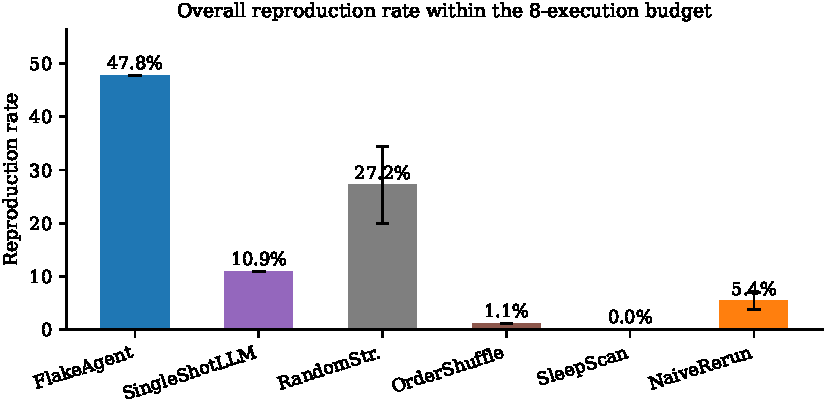
\includegraphics[width=0.92\columnwidth]{figures/repro_overall.pdf}
\caption{Overall reproduction rate: FlakeAgent vs.\ five baselines sharing
the 8-execution budget. Error bars on RandomStrategy, OrderShuffle, and
FlakeAgent are $\pm$ std over 3 seeds on the 30-test variance subset.}
\label{fig:repro-overall}
\end{figure}

\paragraph{Per-category.} Table~\ref{tab:main-results} and
Figure~\ref{fig:repro-category} break reproduction down by category. The
agent's advantage is concentrated where plain rerunning cannot help: it
reproduces every NIO test (via T2) and most ID tests (via T12), categories
where only deliberate execution schemes can expose the failure at all. OD is
the weakest category, as most of its failures trace to cross-class polluters
whose source the agent never sees (Section~\ref{sec:discussion}).

\begin{table}[t]
\caption{Reproduction rates (\% of gate-passed tests) overall and per
category. Best per row in bold, second underlined.}
\label{tab:main-results}
\small
\begin{tabular}{@{}lrrrrrr@{}}
\toprule
 & \textbf{FlakeAgent} & \textbf{NaiveRerun} & \textbf{RandomStr.} &
 \textbf{OrderShuffle} & \textbf{SleepScan} & \textbf{SingleShot}\\
\midrule
Overall & 47.8 & 5.4 & 27.2 & 1.1 & 0.0 & 10.9\\
OD & 20.0 & 0.0 & 15.0 & 5.0 & 0.0 & 5.0\\
TD & 12.9 & 16.1 & 3.2 & 0.0 & 0.0 & 9.7\\
NIO & 100.0 & 0.0 & 84.0 & 0.0 & 0.0 & 24.0\\
ID & 68.8 & 0.0 & 0.0 & 0.0 & 0.0 & 0.0\\
\bottomrule
\end{tabular}
\end{table}

\begin{figure}[t]
\centering
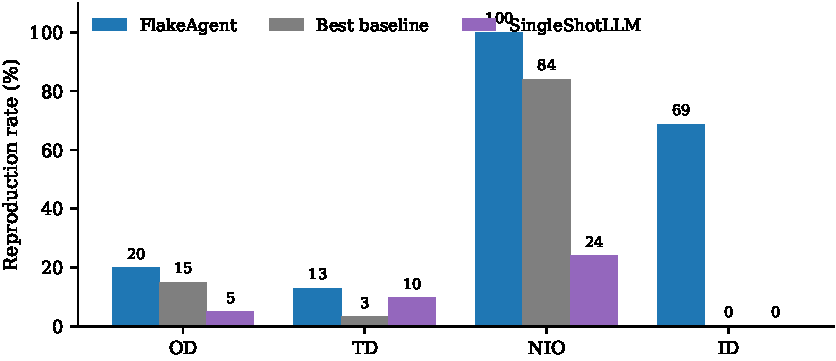
\includegraphics[width=0.92\columnwidth]{figures/repro_category.pdf}
\caption{Reproduction rate by flakiness category (FlakeAgent vs.\ the best
non-agent baseline and SingleShotLLM).}
\label{fig:repro-category}
\end{figure}

\paragraph{Which strategies reproduce what.}
Figure~\ref{fig:heatmap} attributes every reproduction to the triggering
strategy, per ground-truth category. The diagonal is clear: all NIO
reproductions come from T2 (same-JVM double run), most ID from T12 (NonDex),
and OD from T5 (polluter--victim); TD scatters across T1, T10, and T12,
consistent with no single strategy dominating. Two reproductions are T12
fault-injection artifacts whose diagnosed category disagrees with the
ground-truth label (one OD, one TD); we flag them in
Section~\ref{sec:threats} and exclude them from the category-accuracy
discussion below. The heat map is a category $\times$ strategy effectiveness
map, of independent value to practitioners choosing a reproducer.

\begin{figure}[t]
\centering
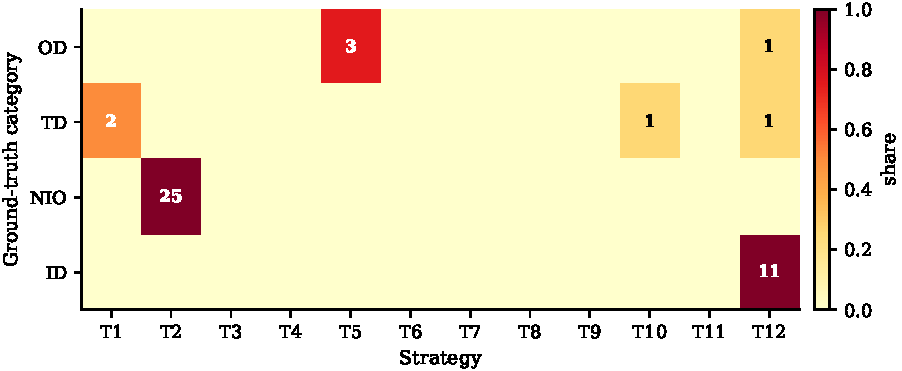
\includegraphics[width=0.95\columnwidth]{figures/heatmap.pdf}
\caption{Category $\times$ strategy reproduction heat map: fraction of
reproductions of each ground-truth category triggered by each strategy
(FlakeAgent runs only).}
\label{fig:heatmap}
\end{figure}

\paragraph{Attempts to reproduction.}
Figure~\ref{fig:atr} (left) shows the ECDF of executions until first
reproduction. FlakeAgent's median ATR is 4.5 executions; 50.0\% of
its reproductions happen within the first 4 executions (i.e., during
or shortly after Step 0 + first planned strategy), and 77.3\% within 5,
with the remainder spread across the loop, evidence of genuine multi-round
search.

\begin{figure}[t]
\centering
\begin{subfigure}[b]{0.48\columnwidth}
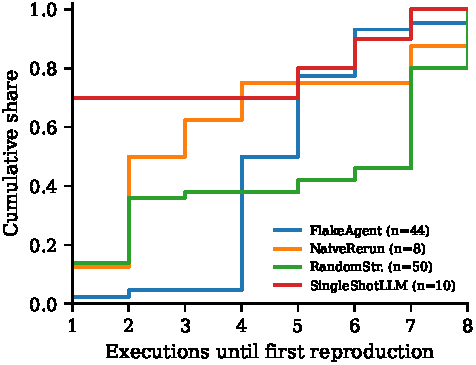
\includegraphics[width=\columnwidth]{figures/atr_ecdf.pdf}
\caption{ECDF of executions until first reproduction.}
\end{subfigure}\hfill
\begin{subfigure}[b]{0.48\columnwidth}
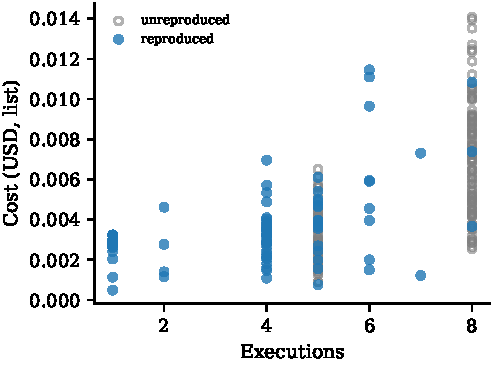
\includegraphics[width=\columnwidth]{figures/cost_scatter.pdf}
\caption{Cost vs.\ attempts per test; reproduced tests in solid, unreproduced
in hollow markers.}
\end{subfigure}
\caption{Search efficiency (left) and cost distribution (right) of
FlakeAgent on the full benchmark.}
\label{fig:atr}
\end{figure}

\subsection{RQ2: Diagnosis accuracy and grounding}
\label{sec:rq2}

On the 44 reproduced tests, the diagnoser commits to a category with
top-1 accuracy 86.4\% exact and 95.5\% coarse (order-dependent vs.\
not). Table~\ref{tab:diagnosis} reports per-category accuracy and, more
importantly, evidence grounding against the developer fix
(\texttt{Fixed.patch}): \emph{evidence precision} is 16.5\% — 17 of 103
cited lines fall inside the fix diff — and \emph{fix-hit} is 36.4\%:
16 of 44 diagnoses cite at least one line the developer changed. The
per-diagnosis \emph{confidence} the model reports correlates moderately with
correctness (Pearson $r = 0.53$; correct diagnoses average 0.86 confidence
vs.\ 0.52 for incorrect ones); we report it but do not rely on it.

\begin{table}[t]
\caption{Diagnosis evaluation on reproduced tests. Evidence is evaluated
against the developer fix diff.}
\label{tab:diagnosis}
\small
\begin{tabular}{@{}lrrrrr@{}}
\toprule
 & \textbf{Diagnosed} & \textbf{Category acc.} & \textbf{Coarse acc.} &
 \textbf{Evid. precision} & \textbf{Fix-hit}\\
\midrule
Overall & 44 & 86.4\% & 95.5\% & 16.5\% & 36.4\%\\
OD & 4 & 50.0\% & 50.0\% & 10.0\% & 25.0\%\\
TD & 4 & 75.0\% & 100.0\% & 10.0\% & 25.0\%\\
NIO & 25 & 100.0\% & 100.0\% & 17.9\% & 40.0\%\\
ID & 11 & 72.7\% & 100.0\% & 18.5\% & 36.4\%\\
\bottomrule
\end{tabular}
\end{table}

\subsection{RQ3: Ablations}
\label{sec:ablation}

Figure~\ref{fig:ablation} and Table~\ref{tab:ablation} report the four
ablations. Removing the reflection loop ($-$reflection) drops reproduction
from 47.8\% to 16.3\% ($-31.5$ pp); shrinking the strategy space ($-$space4)
to 12.0\% and withholding source ($-$source) to 8.0\% on the 50-test subset
(vs.\ 46.0\% for the main config). The gains trace to the reflection loop,
the strategy-space breadth, and source grounding, each contributing
measurably. The Warm configuration isolates the reproduction loop: with the
failure given, the diagnoser commits to a category on 36.0\% of tests (lower
than the 86.4\% cold-start, as a minority of warm replies were unparseable,
Section~\ref{sec:threats}), with evidence grounding comparable to cold-start.

\begin{table}[t]
\caption{Ablations (reproduction \%, diagnosis metrics on each config's own
reproduced subset). $-$reflection runs on the full benchmark; $-$space4,
$-$source, and Warm run on the 50-test stratified subset.}
\label{tab:ablation}
\small
\begin{tabular}{@{}lrrrrr@{}}
\toprule
\textbf{Config} & \textbf{Repro.} & \textbf{Category acc.} &
\textbf{Evid. precision} & \textbf{Fix-hit} & \textbf{\$/test}\\
\midrule
FlakeAgent (main) & 47.8\% & 86.4\% & 16.5\% & 36.4\% & 0.0066\\
$-$reflection & 16.3\% & 80.0\% & 16.1\% & 26.7\% & 0.0032\\
$-$space4 & 12.0\% & 83.3\% & 25.0\% & 50.0\% & 0.0075\\
$-$source & 8.0\% & 100.0\% & 11.1\% & 25.0\% & 0.0053\\
Warm & n/a & 36.0\% & 16.0\% & 12.0\% & 0.0024\\
\bottomrule
\end{tabular}
\end{table}

\begin{figure}[t]
\centering
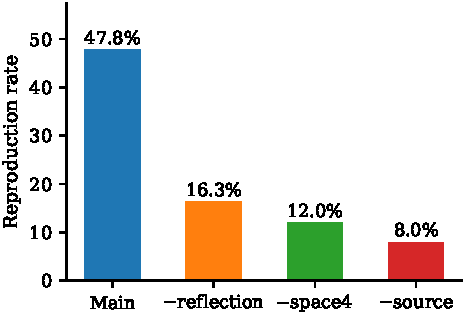
\includegraphics[width=0.92\columnwidth]{figures/ablation.pdf}
\caption{Ablation results: reproduction rate for the four ablations vs.\
the main configuration.}
\label{fig:ablation}
\end{figure}

\subsection{RQ4: Cost}
\label{sec:cost}

Table~\ref{tab:cost} and Figure~\ref{fig:atr} (right) report the cost
profile. At \$0.006 USD median per test (list prices), reproducing one flaky
failure costs \$0.014 USD on average; the distribution is right-skewed
(median \$0.0066, p90 \$0.01) because the loop is budget-bounded rather than
cost-bounded, and wall-clock follows the same pattern (median 1.55 min, p90
3.71 min). The whole 92-test benchmark costs \$0.60 USD in total. By
comparison, the dataset's own validation gate runs up to 10 official-mechanism
invocations per test, each an order of magnitude slower than one agent
execution; FlakeAgent reproduces the same failures at under a cent per test,
and adds a diagnosis no rerun loop can provide.

\begin{table}[t]
\caption{Cost profile of FlakeAgent (main configuration, full benchmark, at
provider list prices; usage from provider-reported metadata).}
\label{tab:cost}
\small
\begin{tabular}{@{}lrrrr@{}}
\toprule
\textbf{Metric} & \textbf{Median} & \textbf{Mean} & \textbf{p90} & \textbf{Total}\\
\midrule
LLM calls per test & 5.0 & 3.95 & 5.0 & 363\\
Executions per test & 8.0 & 6.43 & 8.0 & 592\\
Input tokens per test & 13{,}833 & 14{,}434 & 27{,}376 & 1{,}327{,}944\\
Output tokens per test & 5{,}932 & 7{,}336 & 13{,}605 & 674{,}927\\
Cost per test (USD) & 0.006 & 0.0066 & 0.01 & 0.60\\
Cost per reproduction (USD) & \multicolumn{3}{c}{--} & 0.014\\
Wall-clock per test (min) & 1.55 & 2.36 & 3.71 & 216\\
\bottomrule
\end{tabular}
\end{table}

\subsection{Cross-model comparison}

Table~\ref{tab:models-results} compares the six models on the stratified
50-test subset under the identical protocol (same prompts, budgets,
temperature; only the model differs). DeepSeek-V4.1-Flash reproduces 46.0\%,
while the other five cluster tightly at 10--12\%. The gap between the best
and worst model (46.0\% vs.\ 10.0\%, 36~pp) is comparable to the gap between
FlakeAgent and its ablations ($-$source 8.0\%), so model choice matters as
much as design choice on this task. The frontier reasoning-heavy models do
not outperform their cheaper sibling here: at low reasoning effort their
visible reply is small and their plan quality suffers
(Section~\ref{sec:setup}). DeepSeek-V4.1-Flash's edge is likely both a
stronger prior and the 4{,}000-token output budget that lets its reasoning
survive the visible-reply cap.

\begin{table}[t]
\caption{Cross-model comparison on the 50-test stratified subset
(reproduction \%, diagnosis, cost per test at list prices).}
\label{tab:models-results}
\small
\begin{tabular}{@{}lrrrrr@{}}
\toprule
\textbf{Model} & \textbf{Repro.} & \textbf{Category acc.} &
\textbf{Evid. precision} & \textbf{Fix-hit} & \textbf{\$/test}\\
\midrule
DeepSeek-V4.1-Flash & 46.0\% & 82.6\% & 18.2\% & 39.1\% & 0.0066\\
DeepSeek-V4-Pro & 12.0\% & 83.3\% & 14.3\% & 16.7\% & 0.0353\\
Gemini-3.8-Flash & 10.0\% & 80.0\% & 28.6\% & 40.0\% & 0.0070\\
Grok-4.7 & 12.0\% & 66.7\% & 12.5\% & 16.7\% & 0.0300\\
GPT-5.6 & 12.0\% & 100.0\% & 0.0\% & 0.0\% & 0.0374\\
GPT-6-Astra & 10.0\% & 100.0\% & 10.0\% & 20.0\% & 0.0928\\
\bottomrule
\end{tabular}
\end{table}

\subsection{Reliability}

On the 30-test variance subset, FlakeAgent's mean reproduction rate across 3
seeds is 28.9 $\pm$ 8.4\% (RandomStrategy: 15.6 $\pm$ 10.2\%, NaiveRerun:
5.6 $\pm$ 1.6\%). The agent's variance is larger than the baselines', which
is expected: its decisions are sampled from an LLM planner, so early-round
strategy choices diverge across seeds; we flag this sampling noise in
Section~\ref{sec:threats}.

\section{Case Studies}
\label{sec:cases}

\subsection{NIO: the same-JVM double run that reruns cannot see}

Our motivating example, \texttt{enums} in \texttt{junit-quickcheck}
(\texttt{quickcheck485}), is also our cleanest NIO case study; its full
trajectory appears in Figure~\ref{fig:case}. Step 0's three isolated reruns
all pass; the planner reads the test source, hypothesizes that nested
JUnitQuickcheck classes leave static accumulators unreset, and selects T2
(\texttt{runs: 2}). Sub-run 1 \texttt{PASS} and sub-run 2 \texttt{ERROR}
(\emph{expected: $<$100$>$ but was: $<$200$>$}) confirm the accumulation. The
diagnoser commits to NIO (confidence 0.98) and cites the static accumulator
(lines~83--90) and the failing assertion (line~460), both inside the region
the developer later fixed. Total cost: 2 LLM calls, 4 executions, 31 seconds,
\$0.0038 — and no rerun-based baseline can ever succeed on this test.

\subsection{OD: static factory state left behind by a sibling test}
\label{sec:case-od}

\texttt{DirectoryManagerFactoryTest\#createDirectoryManagerIoException} in
\texttt{wikidata-toolkit} (\texttt{wdtk-util}) is our cleanest OD case. The
victim expects \texttt{IOException} from
\texttt{DirectoryManagerFactory.createDirectoryManager("/nonexistent/...", true)}
when the factory is configured with the real
\texttt{DirectoryManagerImpl}, which validates the path and throws. Step 0's
three isolated reruns all pass: in isolation the test always installs the
right manager class. The planner reads the two sibling tests and forms the
hypothesis that the factory's \emph{static} manager class is the shared
state: \texttt{createDirectoryManagerNoConstructor} calls
\texttt{setDirectoryManagerClass(TestDirectoryManager.class)}, and the inner
\texttt{TestDirectoryManager} has no \texttt{(Path, boolean)} constructor, so
a subsequent \texttt{createDirectoryManager} reflection call fails with
\texttt{RuntimeException} instead of reaching the \texttt{IOException} path.
It selects T5 with exactly that polluter; the victim then fails on the first
attempt. The diagnoser commits to OD with confidence 0.98 and grounds the
diagnosis in three evidence sites --- the polluter's mutation of the static
field (lines~111--113), the polluting \texttt{TestDirectoryManager}'s
constructor set (lines~37--83), and the victim's
\texttt{@Test(expected=IOException.class)} assertion (lines~116--119).
The developer's fix confirms the mechanism exactly: a
\texttt{@Before} hook resets the manager class to
\texttt{DirectoryManagerImpl.class} before every test. Two LLM calls, four
executions, 21.5 seconds, \$0.0023. NaiveRerun can never observe this failure
(no single run fails); OrderShuffle would need the one specific polluter to
precede the victim within its randomized order, which the agent instead
targets directly from source evidence.

\subsection{TD: a timing race reproduced by parallel execution, not the injected sleep}
\label{sec:case-td}

\texttt{TestInstallSnapshotNotificationWithGrpc\#testInstallSnapshotNotificationCount}
in \texttt{ratis} (\texttt{RATIS-1363}) shows the loop reaching a TD failure
by a route the dataset's own patch does not. The test boots a
\texttt{MiniRaftCluster} over gRPC and asserts that exactly 20
\texttt{InstallSnapshotNotification} events arrive
(\texttt{assertEquals(expectedNotificationCount, notificationCount.get())},
line~280). Step~0's three isolated reruns all pass. The planner's first
hypotheses target timing and shared state: T7 (CPU/IO stress, two cpus) fails,
T2 (same-JVM double run) fails, and T6 injects a 500\,ms sleep at the entry of
the \emph{test method} — the only method name visible cold-start — which also
fails, because the sensitivity lives in the asynchronous gRPC delivery path in
production code, not in the test body. After a second, heavier stress attempt
(four cpus), the planner switches family to T10 (parallel class execution,
four threads) and the assertion fails: \emph{expected $<$20$>$ but was
$<$19$>$}. The diagnoser commits to TD with confidence 0.6 and cites three
sites in the test class — the cluster bootstrap (line~252), the failing count
assertion (line~280), and the gRPC transport subclass that delivers
notifications on separate threads — matching the mechanism. Notably, the
dataset's own reproduction patch for this test injects
\texttt{Thread.sleep} into \texttt{BaseStateMachine} in \emph{production}
code; the agent instead reproduced the race through a transport-level
perturbation it derived from the failure, without ever seeing that patch.
Six LLM calls, eight executions, 73\,s, \$0.0037.

\begin{figure}[t]
\centering
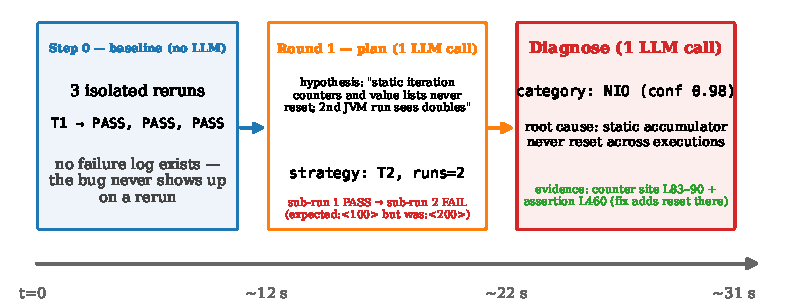
\includegraphics[width=0.9\columnwidth]{figures/case_timeline.pdf}
\caption{Decision timeline of FlakeAgent on the \texttt{enums} NIO case:
each round's hypothesis, strategy, observation, and the final diagnosis with
its evidence.}
\label{fig:case}
\end{figure}

\section{Discussion}
\label{sec:discussion}

\paragraph{The loop and the model both matter.}
The gap between FlakeAgent and SingleShotLLM — same model, same budget, no
loop — isolates the contribution of observation-feedback iteration: 47.8\%
drops to 10.9\% (Section~\ref{sec:rq1}), a 36.9~pp loss. A one-shot planner
proposes the \emph{most likely} strategy a priori; FlakeAgent's value is in
converting a wrong first guess into information (a structured observation:
exit code, assertion, duration) and re-planning against it. The ablation
(Section~\ref{sec:ablation}) and cross-model (Section~\ref{sec:results})
results together show that both the loop and the model matter: removing
source grounding costs 39.8~pp, and switching from the main model to a
frontier sibling costs 35.8--37.8~pp. The method is necessary but not
sufficient — on this task the planner's prior quality, not just the loop
architecture, determines the ceiling.

\paragraph{Where cold-start reproduction still fails.}
Our per-category results isolate the agent's weakest point: order-dependent
tests whose polluter lives in a \emph{different} test class than the victim.
When the polluter is a sibling method (Section~\ref{sec:case-od}), its
mutation is visible in the victim's own source and the agent names it
precisely; when it sits in another class, the planner sees only the class
\emph{name}, not its source, so it guesses a polluter blindly. This is a
failure of perception, not reasoning: the loop has no ``read an arbitrary
file'' action, and adding one is the single highest-leverage extension we see.
The second weak point is time-dependence whose sensitivity sits in
\emph{production} code rather than the test body: cold start, the
sleep-injection strategy can only name methods it sees (the test method and
its helpers), so it misses the asynchronous production path where the race
lives. It can still succeed when a \emph{broad} perturbation widens the race
(Section~\ref{sec:case-td}); but this is the exception, which explains why TD
joins OD as the categories where rerun-free reproduction is genuinely hard.
The fix is the same: let the planner follow a stack trace or synchronization
primitive into production source before choosing a perturbation target.

\paragraph{The strategy map is reusable knowledge.}
Figure~\ref{fig:heatmap} is more than an evaluation artifact: it is an
empirical category $\rightarrow$ strategy effectiveness map, built cold-start
without failure logs, that a CI system with no failure log can consult to
pick a reproducer by category priors. As the warm ablation shows, the same
agent seeded with a pasted log becomes a diagnosis tool comparable to
log-based work like TDRepro~\cite{chen2024tdrepro} — reproduce cold, diagnose
warm.

\paragraph{Cost and CI practice.}
At 0.006 USD and 1.55 minutes per test (median), running FlakeAgent costs
less than a developer's first ``re-run'' coffee break, and the budget caps
make it a predictable, parallelizable CI job. Three design choices keep the
cost low: Step 0 reruns are LLM-free; observations are compressed structures;
and only the last two observations enter the planner context.

\paragraph{Reproduction is the bottleneck, and the loop is portable.}
Our results put a number on a folk claim: of reproduce and diagnose,
reproduction is the hard step — the loss from cold start is dominated by
reproduction failures, not diagnosis quality (warm ablation,
Section~\ref{sec:ablation}). Tools that assume a log exists solve the easier
half; making the bug happen is what FlakeAgent automates. The loop is also
portable: the planner reasons over source and observations while the executor
wraps the project's own test driver, so porting to pytest or Jest means only
reimplementing the twelve strategies — the prompt, loop, anti-degeneracy
rules, and diagnosis protocol carry over unchanged (the benchmark, however,
is Java-only, Section~\ref{sec:threats}).

\section{Threats to Validity}
\label{sec:threats}

\paragraph{Internal.} The main FlakeAgent runs are single-seeded; agent
decisions are stochastic, so single-run rates carry sampling noise, which we
mitigate with a 3-seed variance subset (Section~\ref{sec:setup}) and fixed
temperature and prompts. The executor is large, hand-built infrastructure;
bugs in strategy implementations or log parsing could bias results, which we
mitigate by grounding strategies against the dataset's own mechanisms (T2
reuses iDFlakies, T12 reuses NonDex) and releasing all logs.

\paragraph{External.} The benchmark is drawn from ReproFlake, which is
Java/Maven-only and skewed toward implementation-dependent tests in its full
distribution; our subset deliberately balances categories, so aggregate
numbers are not a statement about ReproFlake's natural distribution. All 116
tests are within one dataset, so results may not transfer to other ecosystems
or proprietary code. All LLM calls use vendor-hosted 2026 models; endpoint
behavior may drift after our runs, which we pin in the artifact.

\paragraph{Construct.} ``Reproduction'' is operationalized as a target-test
failure within budget, judged by the observation probe; a probe parsing bug
could miscount. A subtler threat: fault-injection strategies can make a test
fail for reasons \emph{orthogonal} to its actual flakiness — e.g., NonDex
(T12) can surface a reflection-linkage error in an order-dependent test, and
an aggressive sleep (T6) or heap cap (T9) can trip an unrelated timeout. Such
a ``failure'' counts as a reproduction even though it is not \emph{the} flaky
failure; we therefore flag, in the artifact, every reproduction whose
diagnosed category disagrees with its ground-truth label. Diagnosis grounding
is measured against the developer fix diff, which may inflate or deflate
precision, bounded by our additional manual assessment. Where we compare
against baselines we use McNemar's test; model comparison is descriptive
(one run per model), and costs are at provider list prices.

\section{Conclusion}

We presented FlakeAgent, a closed-loop LLM agent that reproduces flaky test
failures from cold start and diagnoses their root cause with evidence grounded
in the failing execution and code. On a 92-test gate-passed benchmark, it
reproduces 47.8\% of failures within 6 LLM calls, 8 executions, and 45
minutes, outperforming every shared-budget baseline and a single-shot LLM
pipeline; ablations show the reflection loop, strategy space, and source
grounding each earn their cost.


\section{Data Availability}
The artifact, including the FlakeAgent implementation, the benchmark manifest
(116 selected tests, 92 gate-passed, 46 project snapshots, fix commits), raw execution logs, LLM cost logs,
and the scripts that produce every figure and table in this paper, is publicly
available at \url{https://zenodo.org/...} (anonymized).

\bibliographystyle{ACM-Reference-Format}
\bibliography{refs}

\end{document}
